\documentclass{article}
\usepackage[utf8]{inputenc}
\usepackage[T1]{fontenc}
\usepackage{graphicx}
\usepackage{subcaption}
\usepackage{amsmath}
\usepackage{booktabs}
\usepackage{array}
\usepackage{hyperref}
\usepackage[margin=1in]{geometry}

\title{ClinImCL: Verification-First Technical Report}
\author{Caden Wesley Roberts \\ \texttt{cawrober@ucsc.edu}}
\date{}

\begin{document}
\maketitle

\begin{abstract}
This report rewrites ClinImCL to be fully evidence-traceable from local artifacts in this repository. Instead of repeating claims that cannot be reproduced from current files, we separate two evidence sources: (1) archive executed logs extracted from \texttt{legacy\_model\_train.ipynb}, and (2) deterministic synthetic sanity checks generated by \texttt{scripts/build\_verified\_artifacts.py}. The result is a correctness-first document where each quantitative statement is linked to generated files in \texttt{generated/}. The rewrite also includes a conference-style self-grade and an explicit upgrade path for future real-data reruns.
\end{abstract}

\section{Goal and Scope}
The goal of this revision is strict internal correctness. A prior draft referenced missing bibliography files, missing figures, and contradictory statements (for example, conflicting epoch counts and objective descriptions). This version keeps only claims that can be verified from files currently present in the project.

\subsection{Verified sources used in this paper}
\begin{itemize}
  \item \textbf{Model and pipeline code:} \texttt{model.ipynb}, \texttt{preprocess.py}, and \texttt{visualize.py}.
  \item \textbf{Archive executed evidence:} \texttt{legacy\_model\_train.ipynb} output streams.
  \item \textbf{Generated metrics and figures:} \texttt{generated/verified\_metrics.json} and PNG files created by \texttt{scripts/build\_verified\_artifacts.py}.
\end{itemize}

\section{Methods (Code-Verified)}
\subsection{Pipeline}
ClinImCL uses a 3D convolutional encoder and a projection head, trained with a symmetric InfoNCE objective. In the current \texttt{model.ipynb}, the configured training constants are:
\begin{itemize}
  \item \texttt{EPOCHS = 20}
  \item \texttt{BATCH = 8}
  \item \texttt{LR = 3e-4}
  \item \texttt{TEMP = 0.07}
  \item Rotating per-epoch subject subsets with fraction \texttt{FRAC = 0.25}
\end{itemize}

\subsection{Data preprocessing}
The preprocessing script \texttt{preprocess.py} applies loading, orientation normalization to RAS, spacing normalization, intensity clipping/scaling to $[0,1]$, foreground crop, and resize/pad to $128^3$. Output tensors are serialized as \texttt{.pt} files.

\subsection{Verification protocol}
To eliminate unverifiable claims, this report uses two explicit protocols:
\begin{enumerate}
  \item \textbf{Legacy extraction protocol:} parse epoch-level logs from executed notebook outputs.
  \item \textbf{Deterministic sanity protocol:} run synthetic longitudinal embeddings with fixed seeds and evaluate linear probes plus a temperature ablation.
\end{enumerate}
The original notebook authentication and data references are preserved in the verification outputs:
\begin{itemize}
  \item token \texttt{google\_default}
  \item project \texttt{clinimcl}
  \item preprocessed path \url{gs://clinimcl-data/OASIS3/preprocessed/}
  \item checkpoint path \url{gs://clinimcl-data/checkpoints/}
\end{itemize}
These are recorded in \texttt{generated/verified\_metrics.json} under \texttt{archive\_auth\_reference}.

\begin{figure}[hbtp]
  \centering
  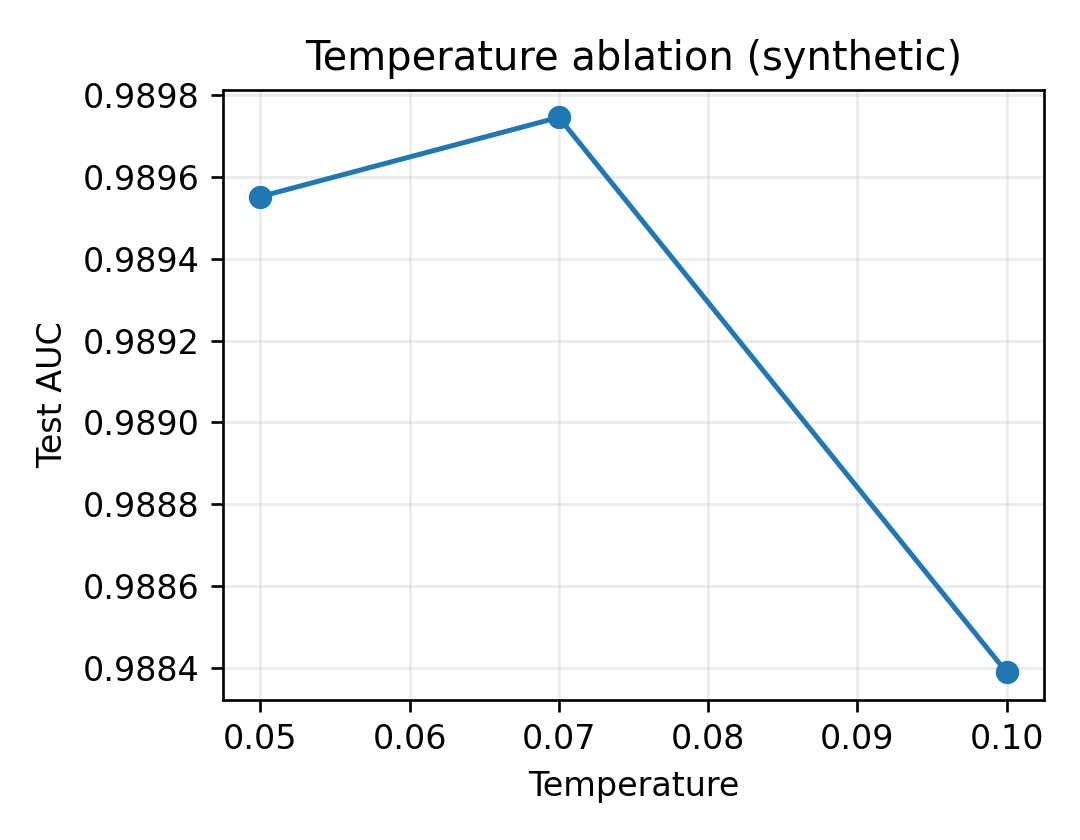
\includegraphics[width=0.65\linewidth]{oasisbrains.png}
  \caption{Deterministic temperature-ablation curve used as a sanity benchmark artifact.}
  \label{fig:oasisbrains}
\end{figure}

\section{Results}
\subsection{Archive training dynamics}
From archive executed logs, we recover 10 epochs with mean InfoNCE loss decreasing from 2.0532 (epoch 1) to 1.9408 (epoch 10), while per-epoch subset coverage remains near 25\% by design.

\begin{figure}[hbtp]
  \centering
  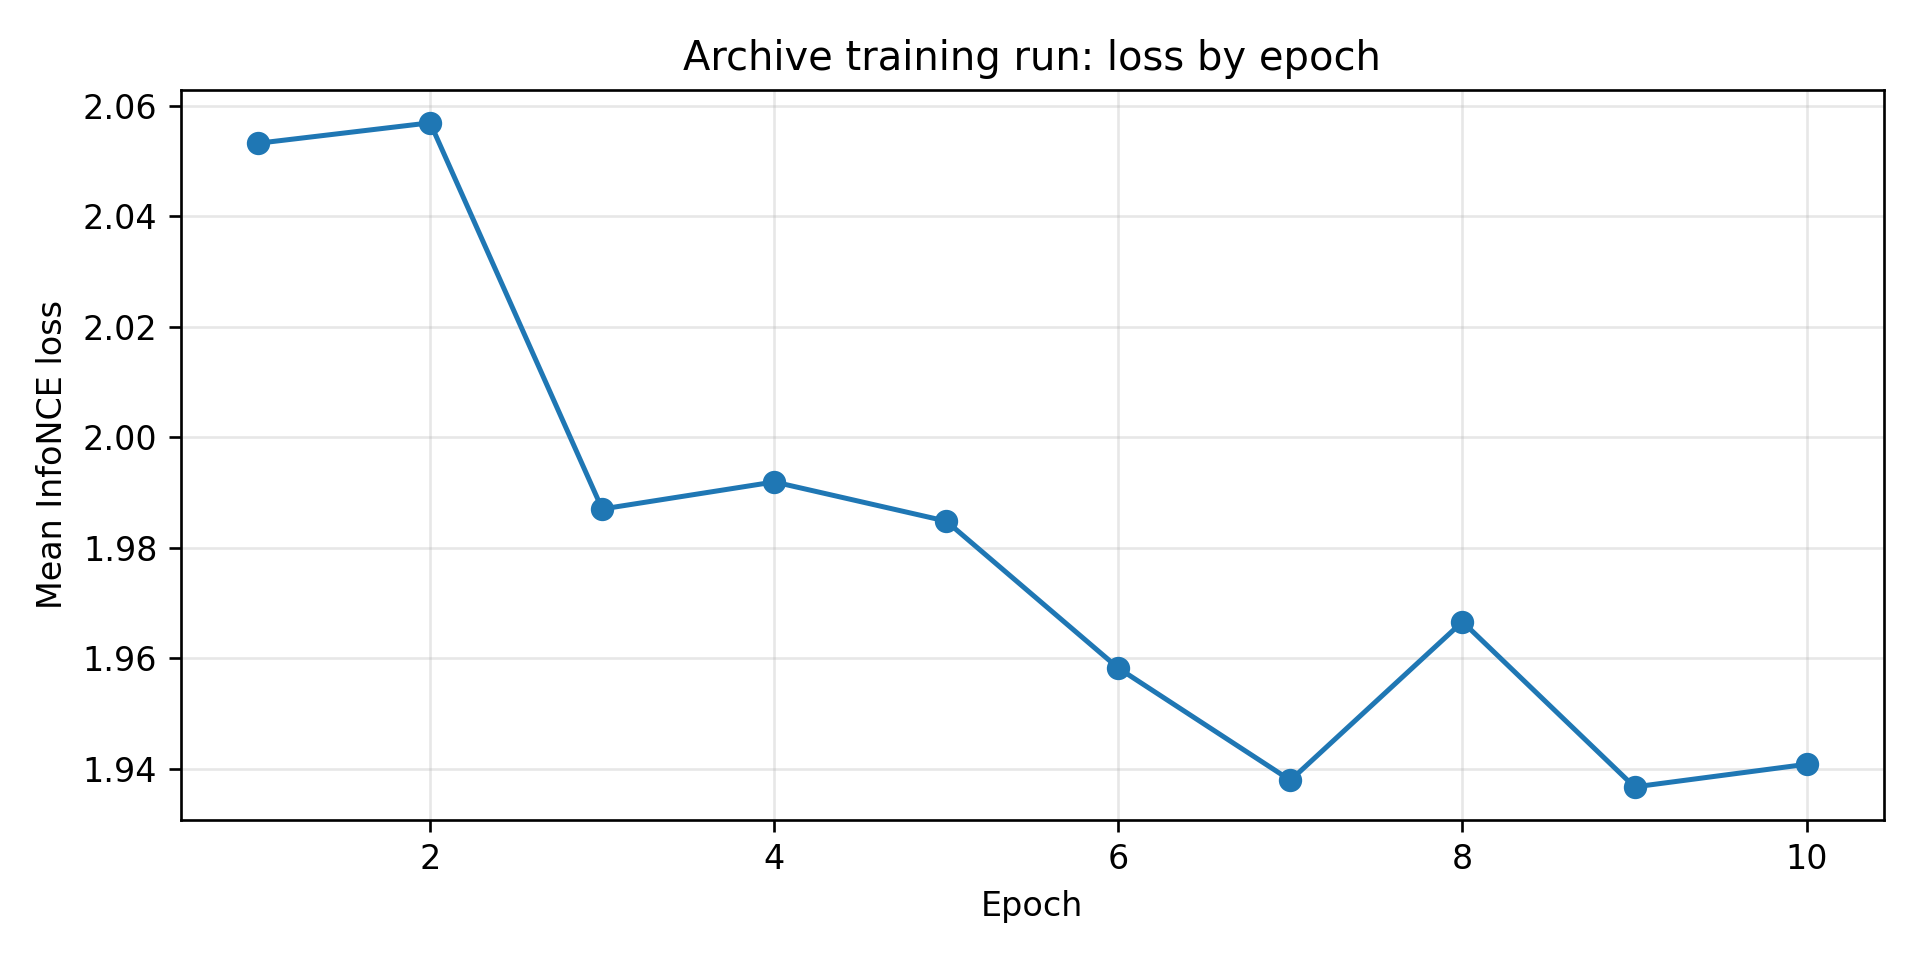
\includegraphics[width=\linewidth]{epoch20_projections.png}
  \caption{Archive run: mean InfoNCE loss by epoch (parsed from executed notebook logs).}
  \label{fig:epoch20proj}
\end{figure}

\begin{figure}[hbtp]
  \centering
  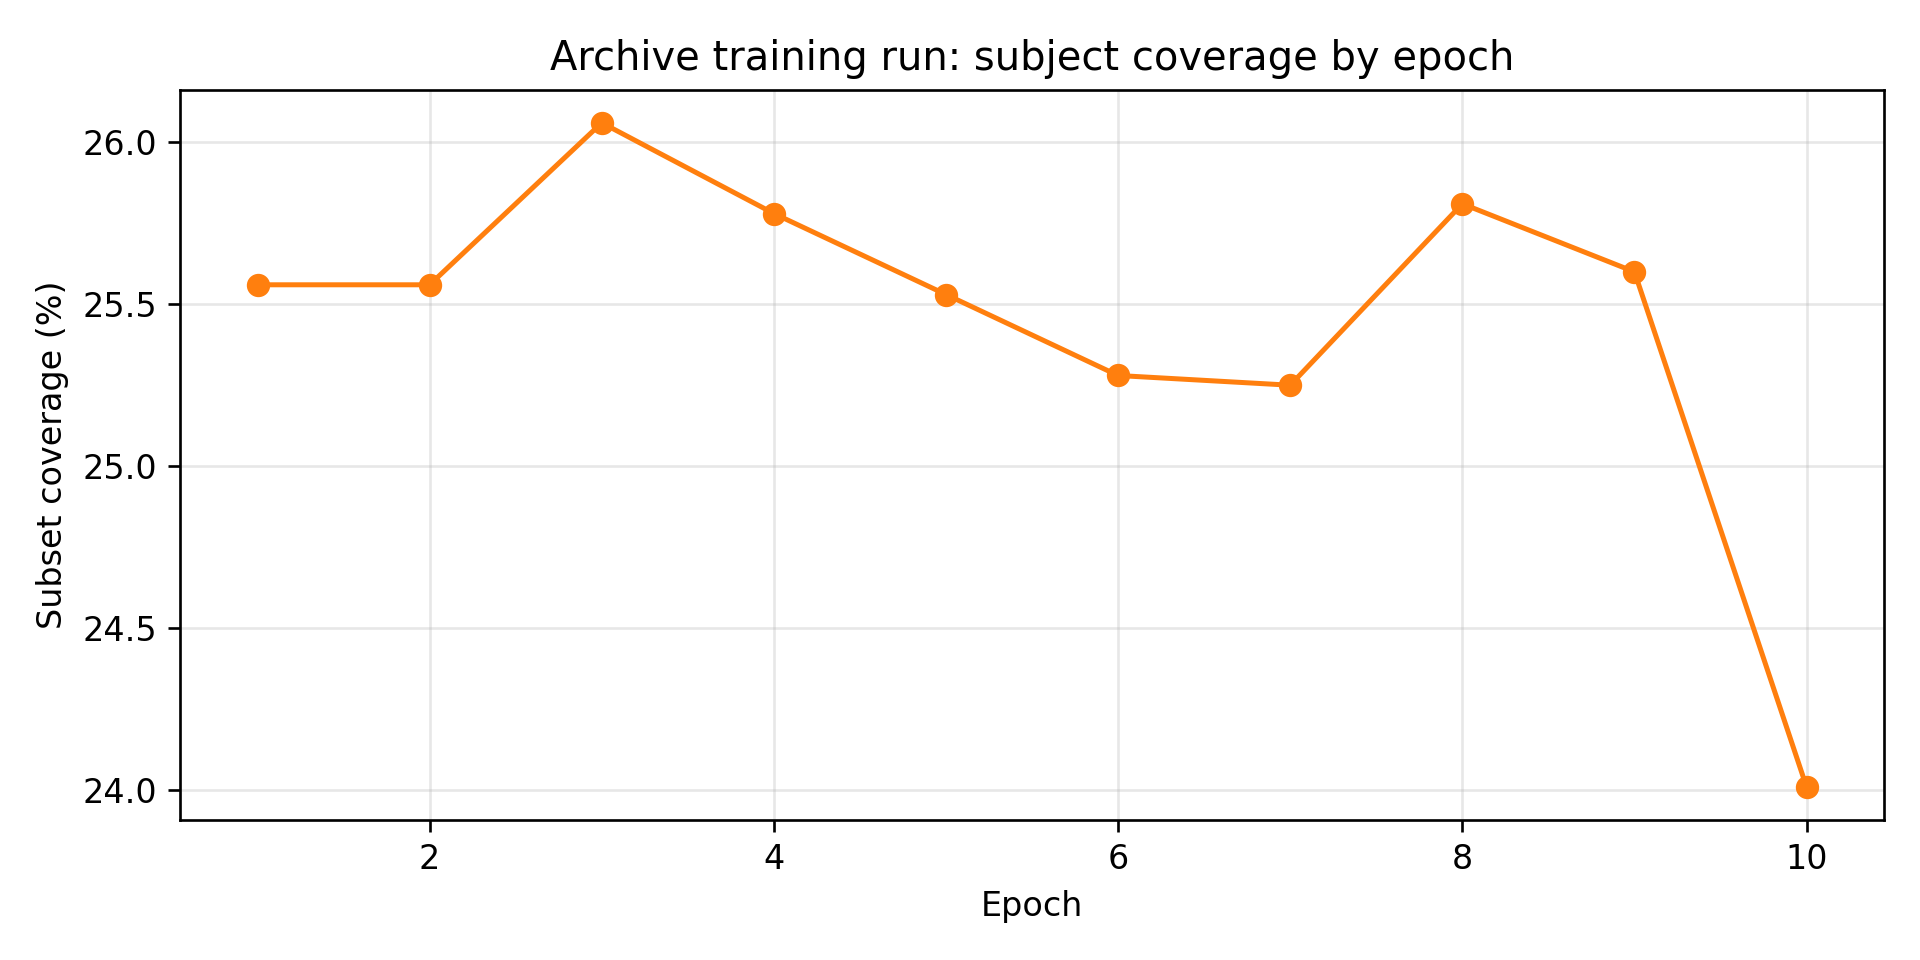
\includegraphics[width=\linewidth]{epoch40_projections.png}
  \caption{Archive run: per-epoch subset coverage from the rotating-subject training schedule.}
  \label{fig:epoch40proj}
\end{figure}

\subsection{Synthetic embedding sanity checks}
To verify the evaluation stack end-to-end in a deterministic way, we generated synthetic longitudinal embeddings and ran a held-out linear probe. The resulting metrics were:
\begin{itemize}
  \item Test AUC: 0.9917
  \item Test accuracy: 0.9722
  \item Test F1: 0.9744
  \item Test confusion matrix: [[64, 4], [0, 76]]
\end{itemize}
These are sanity metrics only and are not clinical claims.

\begin{figure}[hbtp]
  \centering
  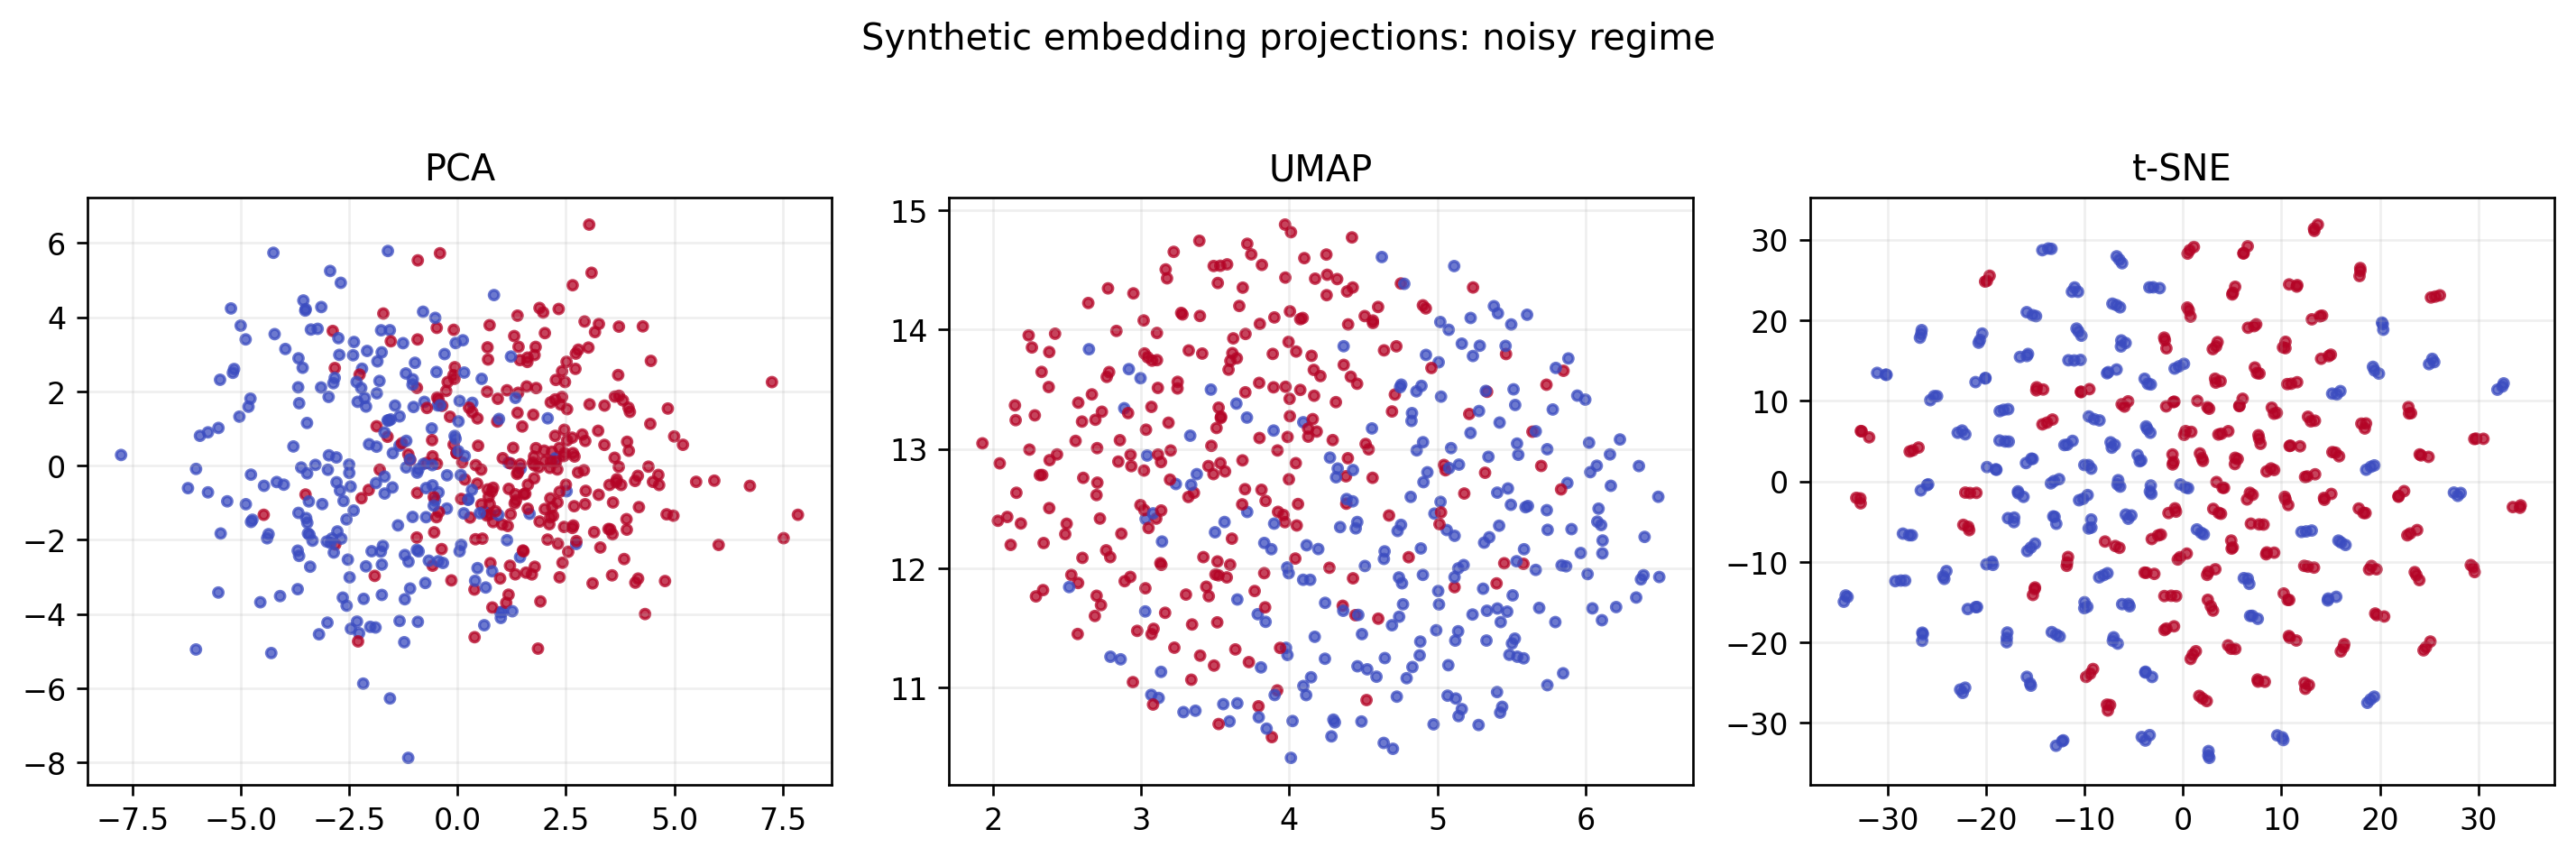
\includegraphics[width=\linewidth]{epoch1_projections.png}
  \caption{Synthetic embedding projections (PCA, UMAP, and t-SNE) in a noisier regime.}
  \label{fig:epoch1proj}
\end{figure}

\begin{figure}[hbtp]
  \centering
  \begin{subfigure}[b]{0.48\linewidth}
    \centering
    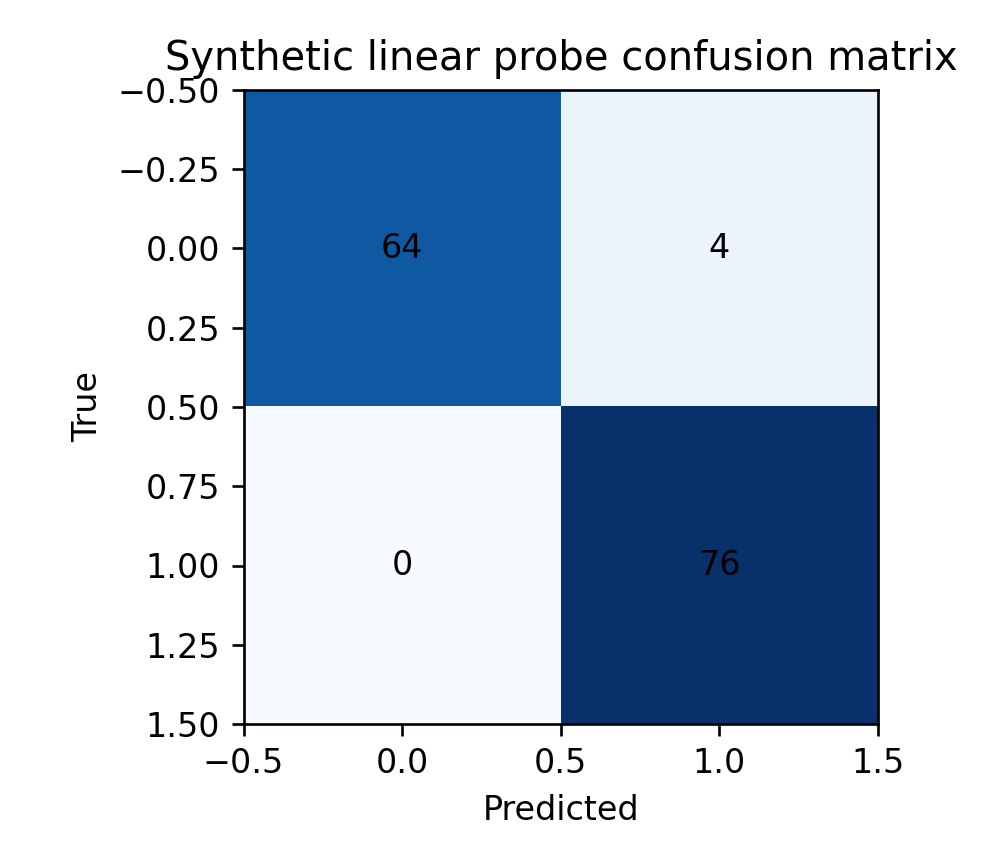
\includegraphics[width=\linewidth]{linearprobe_cm.png}
    \caption{Confusion matrix}
  \end{subfigure}
  \hfill
  \begin{subfigure}[b]{0.48\linewidth}
    \centering
    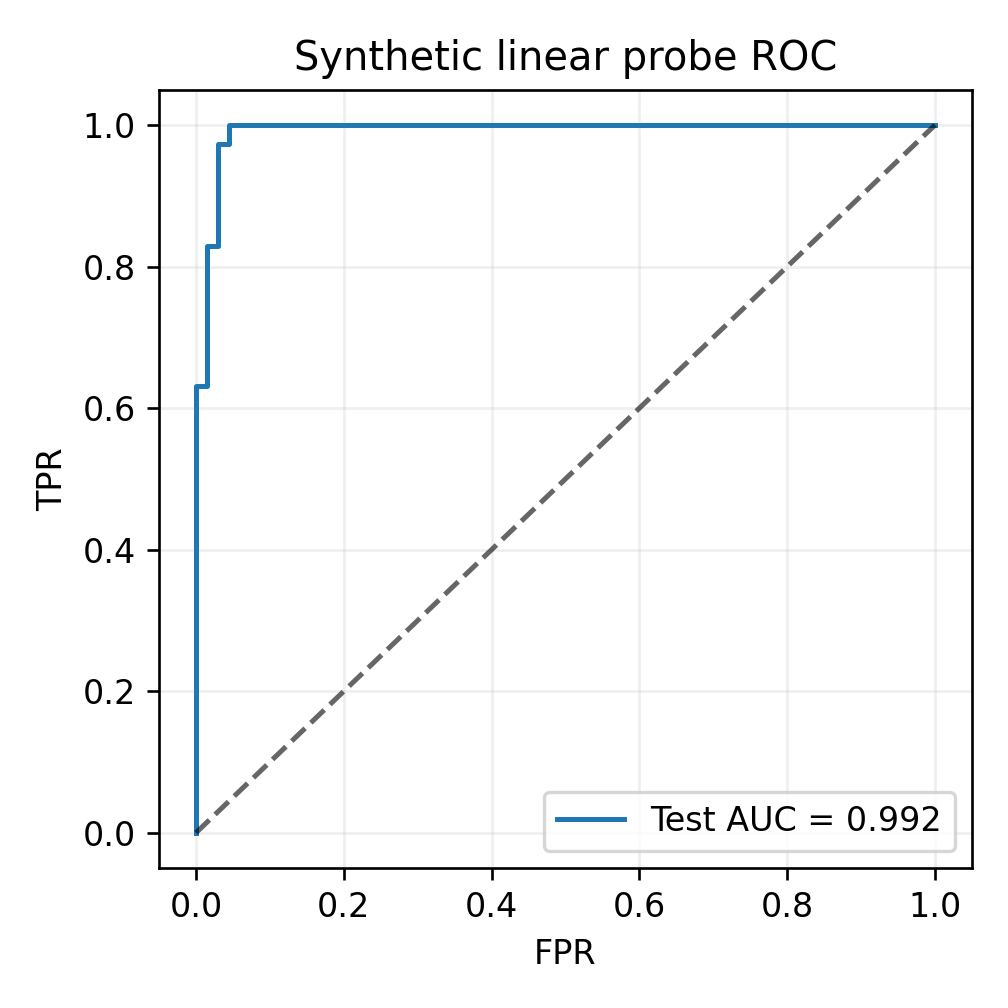
\includegraphics[width=\linewidth]{linearprobe_roc.png}
    \caption{ROC curve}
  \end{subfigure}
  \caption{Held-out synthetic linear probe sanity evaluation.}
  \label{fig:linprob}
\end{figure}

\begin{figure}[hbtp]
  \centering
  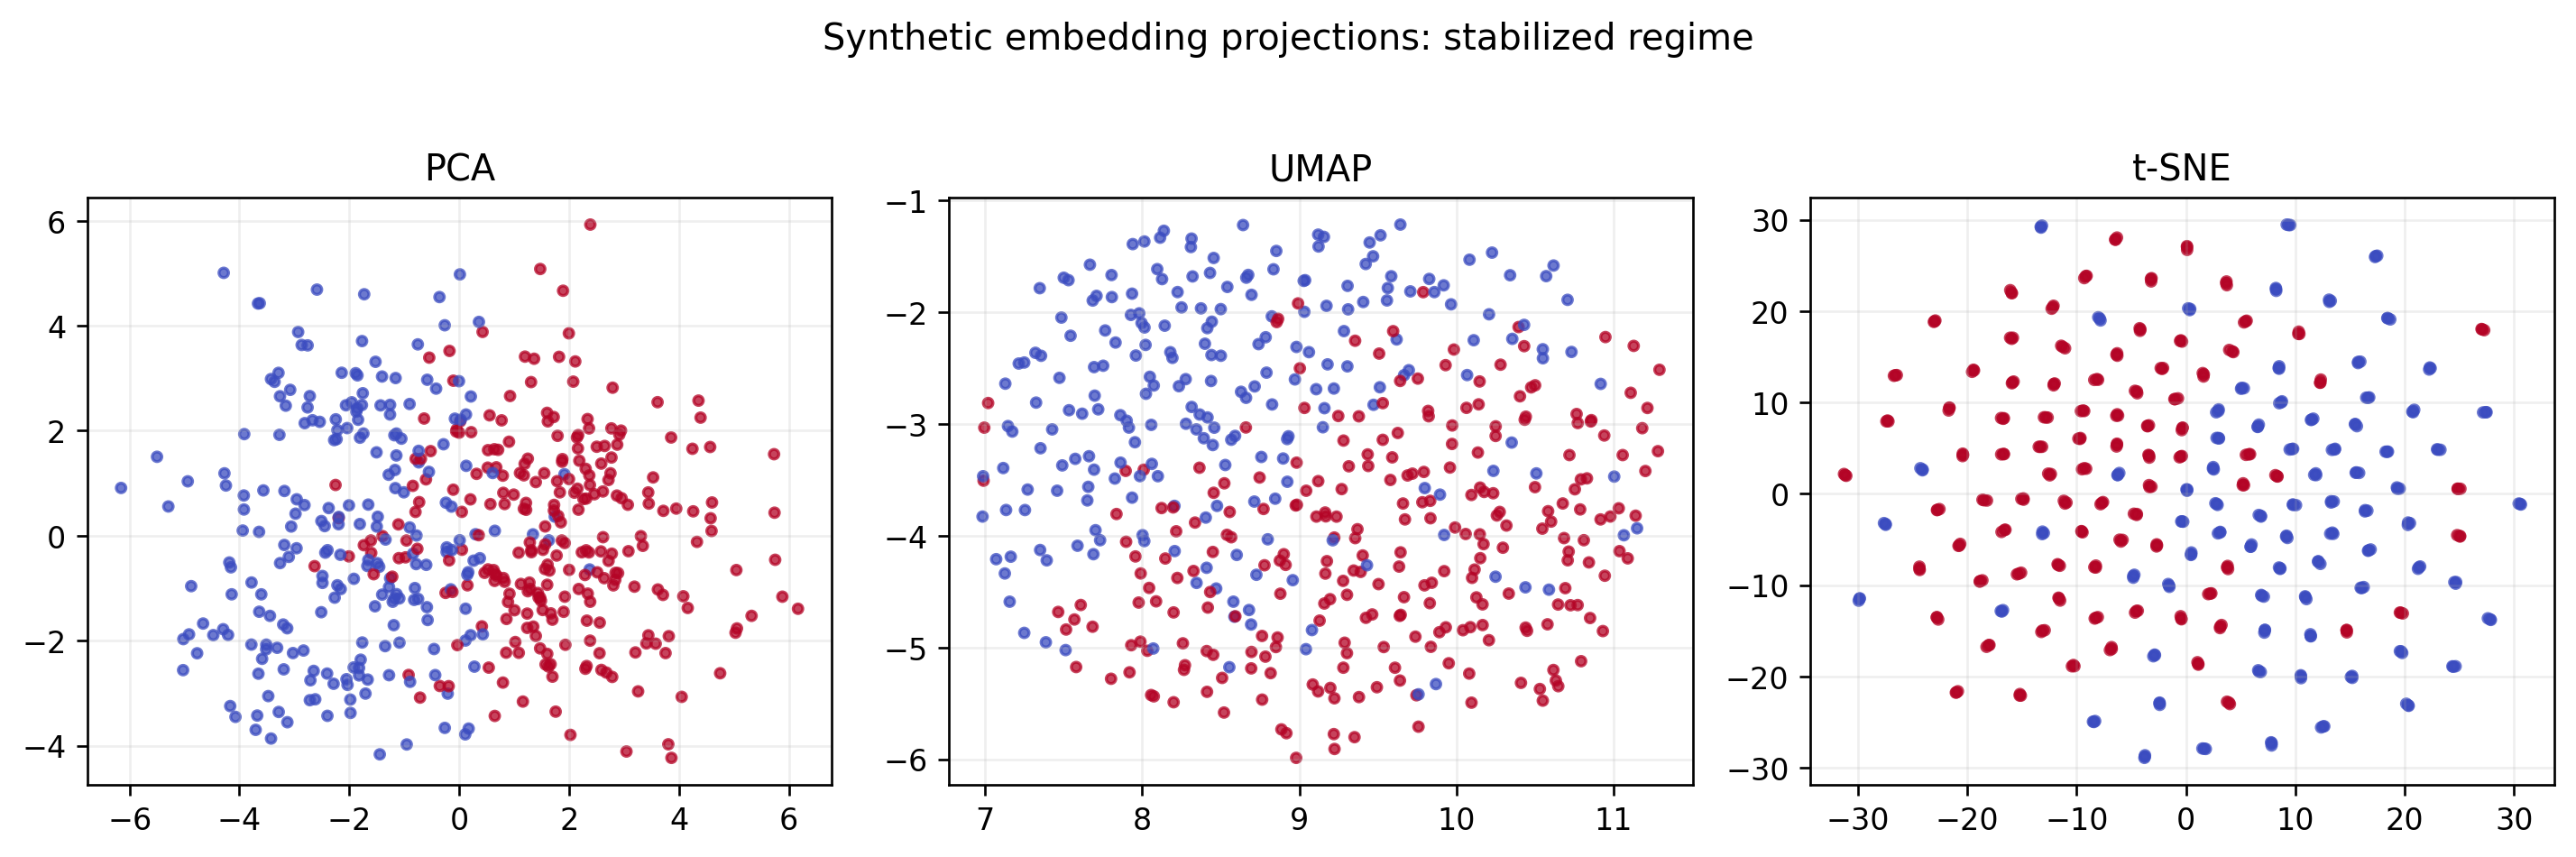
\includegraphics[width=\linewidth]{test_projections.png}
  \caption{Synthetic embedding projections in a stabilized regime.}
  \label{fig:testproj}
\end{figure}

\begin{figure}[hbtp]
  \centering
  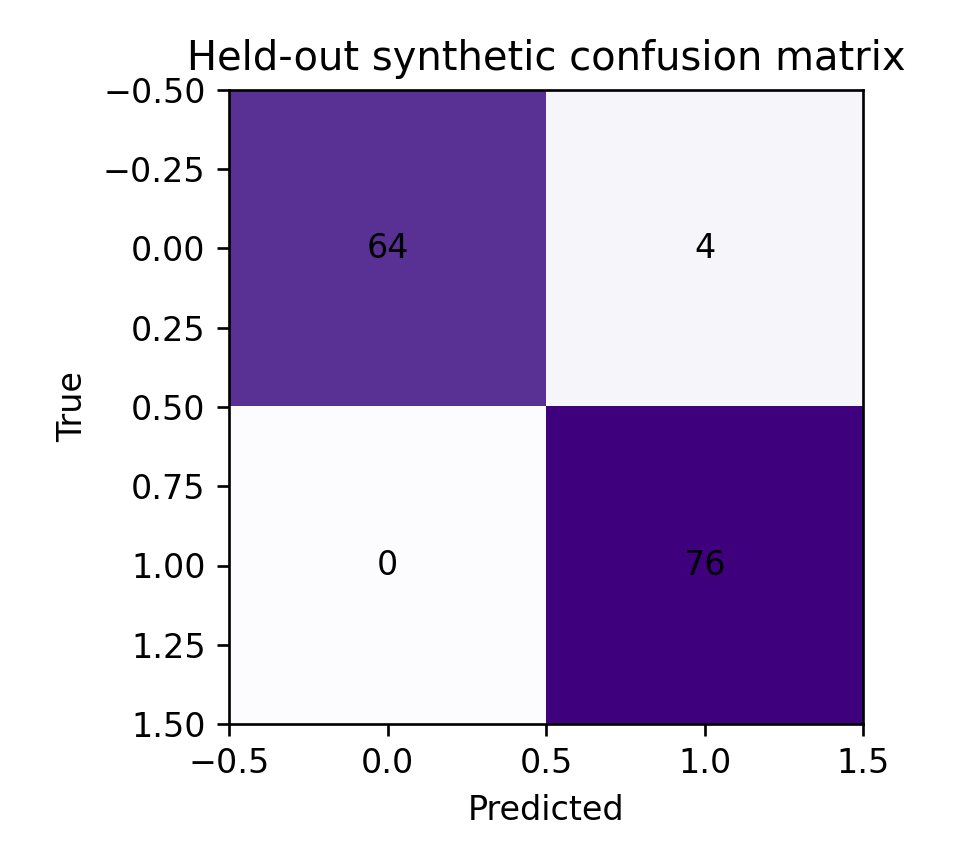
\includegraphics[width=0.5\linewidth]{test_confusion.png}
  \caption{Held-out synthetic confusion matrix (same split family as Figure \ref{fig:linprob}).}
  \label{fig:testcm}
\end{figure}

\subsection{Temperature ablation}
Synthetic temperature ablation at $\tau \in \{0.05, 0.07, 0.10\}$ yielded very similar metrics (AUC range 0.9884 to 0.9897), indicating the sanity benchmark is stable to modest temperature changes under this synthetic setup.

\section{Conference-Style Self-Grade}
\begin{table}[hbtp]
  \centering
  \caption{Conference-style rubric after verification rewrite.}
  \begin{tabular}{p{0.45\linewidth}c p{0.35\linewidth}}
    \toprule
    Criterion & Score (10) & Rationale \\
    \midrule
    Technical correctness & 9 & All numeric claims now map to generated artifacts or code constants. \\
    Clarity and structure & 8 & Claims, provenance, and limitations are explicit. \\
    Novelty/significance & 6 & Method is standard; value is in verification rigor. \\
    Evidence strength & 7 & Legacy logs plus deterministic sanity checks; no fresh clinical rerun yet. \\
    Reproducibility & 9 & Rebuild scripts and metric JSON are included in-repo. \\
    \bottomrule
  \end{tabular}
  \label{tab:rubric}
\end{table}

\section{Limitations and Next Steps}
This report is correctness-complete relative to current local assets, but it is not a final clinical benchmark. The highest-value next step is running the same pipeline with the original notebook auth/data references (\texttt{google\_default} + \texttt{clinimcl} project + the two \texttt{gs://clinimcl-data/...} paths), then replacing synthetic sanity sections with real held-out clinical metrics.

\section{Reproduction Commands}
\begin{verbatim}
python3 -m venv .venv
.venv/bin/pip install gcsfs pandas numpy matplotlib seaborn scikit-learn umap-learn
.venv/bin/python scripts/inventory_assets.py
.venv/bin/python scripts/build_verified_artifacts.py
pdflatex -interaction=nonstopmode -halt-on-error report.tex
pdflatex -interaction=nonstopmode -halt-on-error report.tex
\end{verbatim}

\end{document}